\chapter{Inleiding}

\section{Situering}\label{sec:situering}

Binnen software engineering is UML\cite{RumbaughJames2005Tuml} een veelgebruikt gereedschap om het domein waarin de software die ontworpen wordt alsook de structuur van de software zelf grafisch weer te geven. Het is voor de ontwerper interessant om uit een tekstuele beschrijving van wat de voorgestelde software moet kunnen de relevante concepten en procedures te halen, die neer te zetten in een diagram en door middel van de verscheidene symbolen aangeboden door UML uit te drukken hoe die concepten en procedures met elkaar interageren. Op deze manier kan een team snel duidelijkheid scheppen in welke doelen ze precies moeten bereiken.

Het is echter makkelijk om het overzicht te verliezen als de gebruikte diagrammen omvangrijk worden. Dit kan een probleem zijn omdat fouten die worden gemaakt in de ontwerpfase en pas laat in het productieproces ontdekt worden kostbaar zijn om recht te zetten. Het komt ook voor dat een ontwerper per vergissing overbodige informatie toevoegt aan een diagram en dat daardoor het diagram minder verstaanbaar wordt.

In deze masterproef beschouwen we in het bijzonder klassediagrammen en sequentiediagrammen\cite{RumbaughJames2005Tuml}.
Een klassediagram beschrijft welke concepten (in deze tekst verder \textit{klasses} genoemd) er bestaan binnen de software. Elk van die klasses kan attributen en operaties hebben. Verder geeft een klassediagram ook weer welke klasses in relatie staan tot elkaar. Deze relaties leggen vast aan welke beperkingen alle mogelijke toestanden van de beschreven software moeten voldoen om beschouwd te worden als correct.
Een sequentiediagram modelleert een bewerking op een klasse. Het toont zogenaamde \textbf{levenslijnen} die instanties van bepaalde klasses voorstellen en een opeenvolging van instructies die levenslijnen uitvoeren op een andere levenslijn. Deze instructies veranderen de toestand van het systeem of roepen een andere sequentiediagram op. Sequentiediagrammen bieden ook als---dan -en lusstructuren aan waarmee men de uitvoeringsvolgorde van de instructies kan beheersen.

\section{Klassediagrammen}

Beschouw volgend klassediagram:

\begin{figure}[H]
	\label{fig:cd}
	\centering
	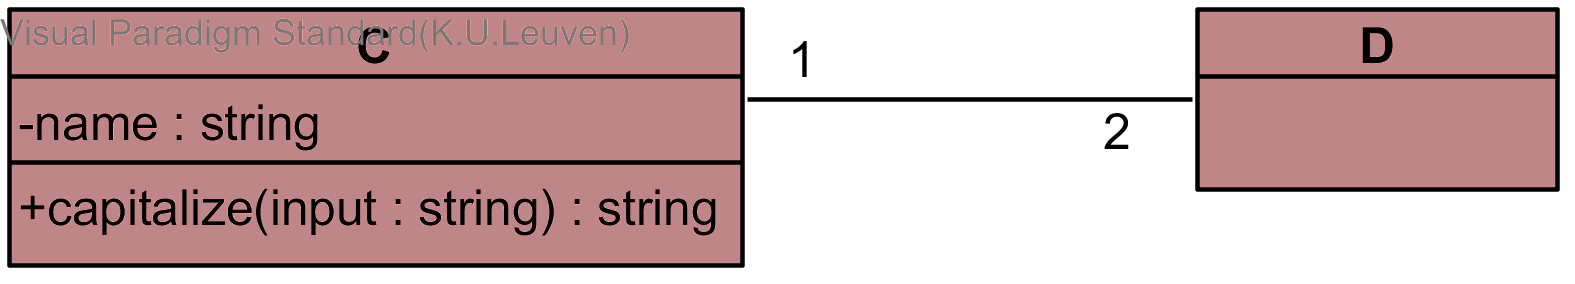
\includegraphics{intro/cd.png}
	\caption{Een voorbeeld van een klassediagram}
\end{figure}

Dit klassediagram drukt uit dat er twee klasses bestaan: \textit{C} en \textit{D}. \textit{C} heeft \'e\'en attribuut, \textit{name}, dat van type \textit{string} is. \textit{D} heeft ook \'e\'en attribuut, \textit{number}, van type \textit{int}. \textit{C} heeft ook \'e\'en operatie \textit{getDNumber} dat \textit{index}, van type \textit{int}, als parameter heeft. \textit{getDNumber} geeft een resultaat terug dat ook van type \textit{int} is. Voorts drukt de lijn tussen \textit{C} en \textit{D} uit dat er een relatie bestaat tussen de twee klasses. Beschouw klasse C. Als we vanuit die klasse de lijn volgen, zien we dat er aan het ander uiteinde staat dat elke \textit{C}-object in relatie moet staan tot exact twee \textit{D}-objecten. Zo ook zien we dat, als we vertrekken vanuit \textit{D}, elk \textit{D}-object in relatie moet staan tot exact \'e\'en \textit{C}-object.
Met de mogelijke problemen genoemd in sectie \ref{sec:situering} in het achterhoofd beschouwen we in deze masterproef twee categorie\"en van gebreken in een klassediagram:

\begin{itemize}
	\item \textbf{Inconsistenties:} Het klassediagram is zo opgebouwd dat geen enkele mogelijke toestand van de software kan beantwoorden aan de voorwaarden die worden opgelegd. Dit betekent dat het stuk van de software dat wordt beschreven in het diagram onmogelijk kan werken.
	\item \textbf{Kwaliteitsgebreken:} Deze gebreken hebben een negatieve impact op de kwaliteit van het softwareontwerp. Zo kunnen ze bijvoorbeeld onduidelijkheden in het ontwerp introduceren of het onderhoud van de software \'e\'enmaal ingezet in productie bemoeilijken.
\end{itemize}

We onderzoeken hoe we klassediagrammen kunnen vertalen naar een voorstelling die ons toelaat om automatisch de consistentie van het diagram te controleren en om kwaliteitsgebreken op te sporen.

\section{Sequentiediagrammen}

Beschouw volgend sequentiediagram:

\begin{figure}[H]
	\label{fig:sd}
	\centering
	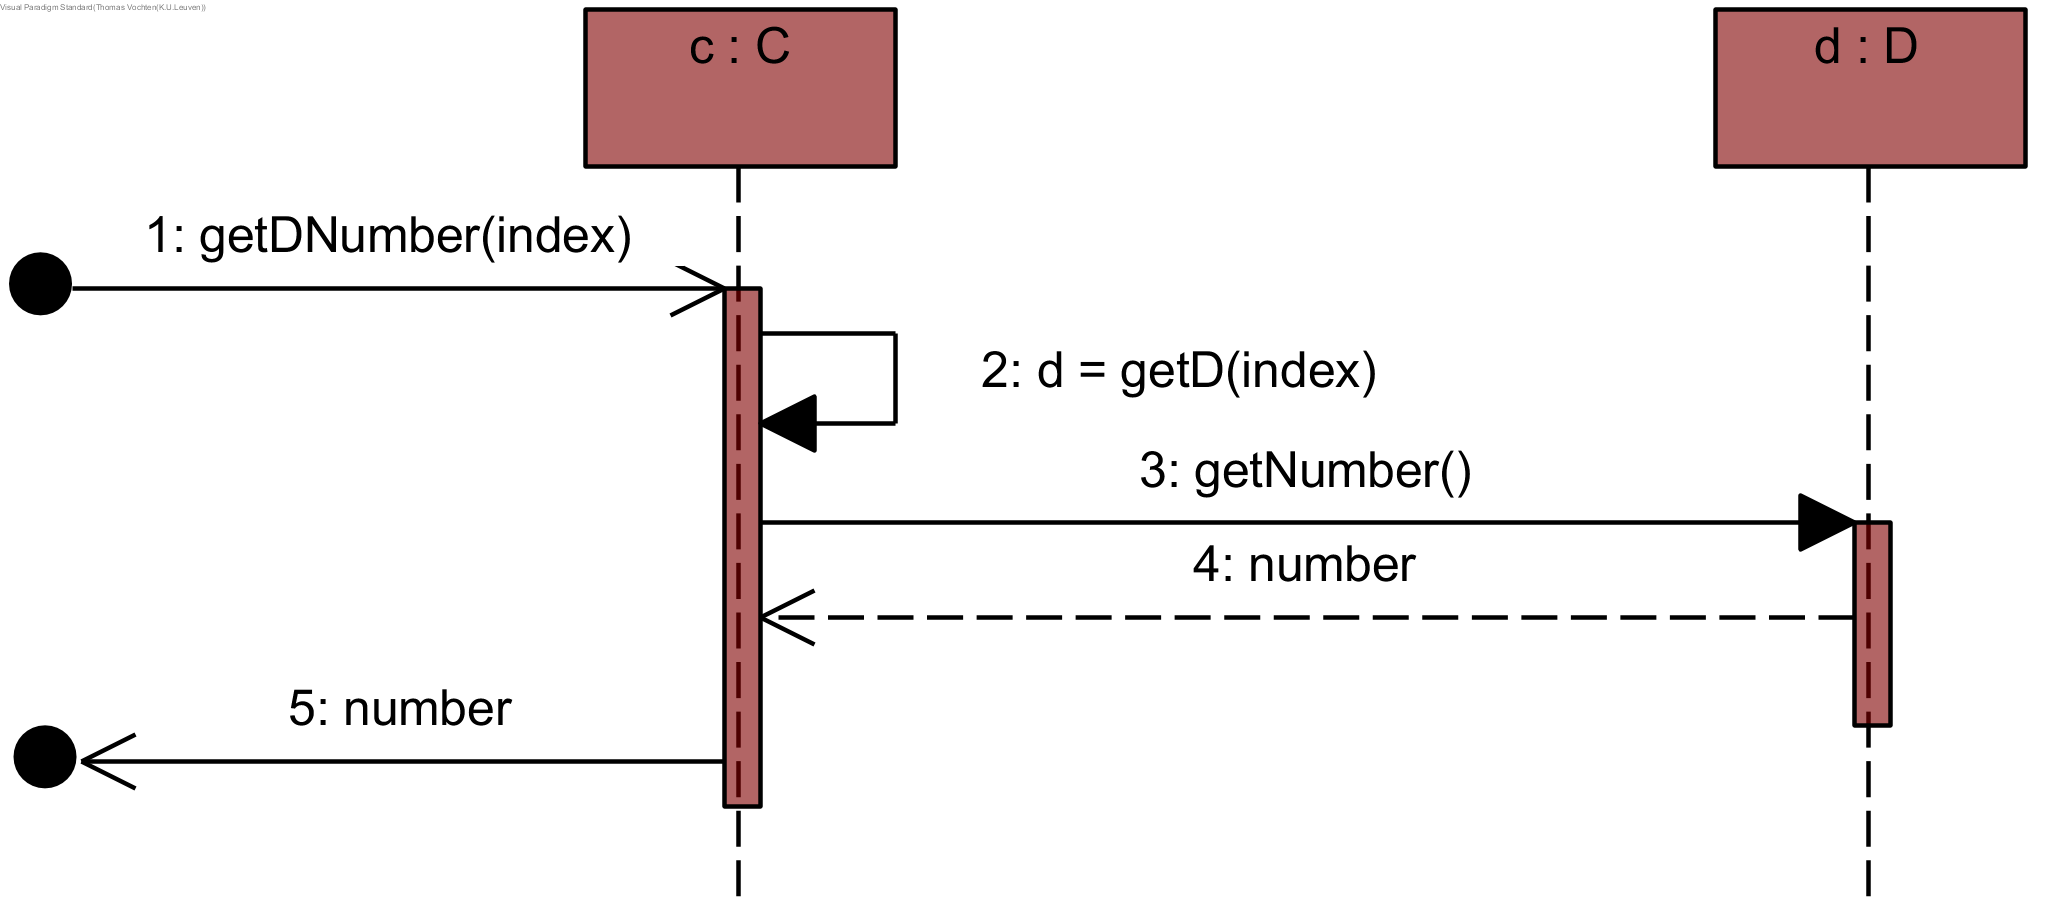
\includegraphics{intro/sd.png}
	\caption{Een voorbeeld van een sequentiediagram}
\end{figure}

Het toont hoe de juiste instantie van \textit{D} wordt opgehaald op basis van invoervariabele \textit{index} en hoe de waarde van het attribuut \textit{number} wordt doorgegeven aan instantie \textit{c}. \textit{c} geeft dan \textit{number} door als uitvoer van het sequentiediagram.

Hoofdstuk \ref{sec:gedrag} bevat een uitgebreider voorbeeld van een sequentiediagram.

In deze masterproef onderzoeken we hoe we sequentiediagrammen kunnen vertalen naar een voorstelling die uitvoerbaar is en of we kunnen verifi\"eren of de uitvoer van een sequentiediagram beantwoordt aan de vereisten voor het deel van het systeem dat dat sequentiediagram modelleert.

\section{Verdere verloop van deze tekst}

We beschouwen logica om een antwoord te zoeken op de vragen gesteld in deze inleiding, meer in het bijzonder FO($\cdot$)\cite{DeCatBroes2014PLaa}, een uitbreiding van predicatenlogica. FO($\cdot$) is een logica die voldoende expressief is voor onze noden en waarvoor software bestaat die theorie\"en kan uitvoeren. We geven eerst een overzicht van de structuur van de rest van deze tekst.

Hoofdstuk \ref{sec:literatuur} geeft een overzicht van literatuur omtrent het gebruik van logica om klassediagrammen en sequentiediagrammen voor te stellen. Hoofdstuk \ref{sec:consistentie} beschrijft hoe we FO($\cdot$) gebruiken om klassediagrammen voor te stellen. Hoofdstuk \ref{sec:kwaliteitsgebrek} beschrijft een alternatieve voorstellingswijze die we gebruiken om bepaalde kwaliteitsgebreken op te sporen. Hoofdstuk \ref{sec:rol-idp} geeft een korte inleiding tot IDP\cite{DeCatBroes2014PLaa}, een kennisbanksysteem voor FO($\cdot$), en beschrijft hoe we IDP gebruiken om te redeneren op de voorstellingswijzen beschreven in de voorgaande hoofdstukken. In hoofdstuk \ref{sec:gedrag} beschrijven we hoe sequentiediagrammen voor te stellen in lineaire tijdscalculus\cite{BogaertsBart2014Sdsu}, een methode om in FO($\cdot$) dynamische systemen te modelleren. In hoofdstuk \ref{sec:evaluatie} evalueren we ons vertalingsproces door een spel te modelleren in een klassediagram en een stel sequentiediagrammen en die diagrammen enerzijds te gebruiken voor een simulatie van het spel en anderzijds om verificaties van gewenste eigenschappen uit te voeren. Daarbij letten we op rekentijd en geheugengebruik. Hoofdstuk \ref{sec:conclusie} geeft een besluit en geeft een aanzet tot verder onderzoek.